%%PREAMBLE-START
\documentclass[sigconf,nonacm]{acmart}
\settopmatter{printfolios=true}
\usepackage{tikz,listings,booktabs,subcaption,array}
\usetikzlibrary{positioning,arrows.meta}
%%PREAMBLE-END
% ---------- LAYOUT KNOBS (tune on Overleaf until both columns of pages 1-2 end flush) ----------
\newcommand{\shotheight}{1.0in}          % height cap of each UI screenshot (Figure 2)
\setlength{\textfloatsep}{8pt plus 2pt minus 2pt}\setlength{\floatsep}{8pt plus 2pt minus 2pt}
\lstset{basicstyle=\ttfamily\fontsize{6.6}{7.6}\selectfont,breaklines=true,columns=fullflexible,keywordstyle=\bfseries,
        frame=single,aboveskip=3pt,belowskip=3pt,xleftmargin=1pt,xrightmargin=1pt,framesep=1.5pt,showstringspaces=false}
\lstdefinelanguage{SQLite}{morekeywords={SELECT,FROM,JOIN,ON,WHERE,GROUP,BY,COUNT,AS,IN,HAVING,ORDER,DISTINCT,UPDATE,SET,DELETE,INSERT,INTO,VALUES,LEFT,IS,NULL},sensitive=false}
\newcommand{\tn}[1]{\texttt{#1}}
\newcommand{\uishot}[2]{\begin{subfigure}[t]{.49\textwidth}\centering
 \includegraphics[width=\linewidth,height=\shotheight,keepaspectratio]{#1}\caption{#2}\end{subfigure}}

\begin{document}
%%FRONT-START
\title{ProduCast: A Relational Model of Film Casting and Production Networks}
\titlenote{Code, SQL scripts and documentation: \url{https://github.com/karanbe17/film-talent-kg}}
% Manual 4.7.1: the graduate student must be listed LAST -- reorder the two \author blocks if needed.
\author{Karan Brahmbhatt}\affiliation{\institution{University of Victoria}\city{Victoria}\state{BC}\country{Canada}}\email{karanbrahmbhatt@uvic.ca}
\author{Moksh Patel}\affiliation{\institution{University of Victoria}\city{Victoria}\state{BC}\country{Canada}}\email{mokshpatel@uvic.ca}

\begin{abstract}
ProduCast maps an ER model of film casting into six SQLite relations seeded with 12 people, 7 movies and 8 cast entries. Keys, \tn{CHECK} constraints and cascading deletes enforce consistent links; a layered Flask app supports searching and editing without SQL. Code and reproducible setup: \url{https://github.com/karanbe17/film-talent-kg}.
\end{abstract}


\maketitle
%%FRONT-END

\section{Introduction}
Flat film lists hide performance roles, repeated collaborations and deletion effects. We translate our ERD into SQLite~\cite{sqlite} using standard SQL features~\cite{iso}, seed known films, and demonstrate CRUD operations through scripts and a Flask interface.

\section{ER-to-Relational Mapping}
Table~3 lists all six relations and constraints. Each uses a surrogate \tn{Id} and named \tn{UK\_}/\tn{FK\_}/\tn{CK\_} constraints. \tn{Person} and \tn{Movie} represent entities; their required, unique names/titles are simplified natural keys that exclude namesakes and remakes. \tn{Actor} and \tn{Director} implement overlapping IS-A subclasses: each has a unique \tn{PersonId} foreign key, and a person may belong to both. \tn{MovieDirector} connects movies to directors; \tn{PerformanceRole} connects movies to actors with \tn{RoleName} and a \tn{RoleType} restricted to Lead, Supporting or Cameo. \tn{UNIQUE(MovieId, ActorId)} permits one role per actor per movie. Cascading foreign keys remove dependent subclass/link rows when their parent is deleted, not unrelated people or movies.

\section{Architecture and Implementation}
Figure~\ref{fig:arch} depicts four layers. Flask routes (\tn{src/ui}) accept forms but contain no SQL. Services (\tn{src/biz}) validate inputs and perform atomic multi-table operations, reporting violations as \tn{BizError}. Parameterized queries and database initialization live in \tn{src/dal}; every connection enables \tn{PRAGMA foreign\_keys = ON}. Paths derive from \tn{\_\_file\_\_} in \tn{src/cmn/config.py} rather than the working directory.

\begin{table}[t]
\caption{Rows loaded by \tn{python main.py}.}\label{tab:rows}
\small\begin{tabular}{@{}llp{1.45in}@{}}\toprule
\textbf{Relation} & \textbf{Rows} & \textbf{Note}\\\midrule
\tn{Person} & 12 & 6 directors, 6 actors\\
\tn{Actor} & 6 & subset of \tn{Person} (IS-A)\\
\tn{Director} & 6 & subset of \tn{Person} (IS-A)\\
\tn{Movie} & 7 & six genres\\
\tn{MovieDirector} & 7 & one director per movie\\
\tn{PerformanceRole} & 8 & 7 Lead, 1 Supporting\\\bottomrule
\end{tabular}
\end{table}

\begin{figure*}[t]
\centering
\resizebox{\textwidth}{!}{%
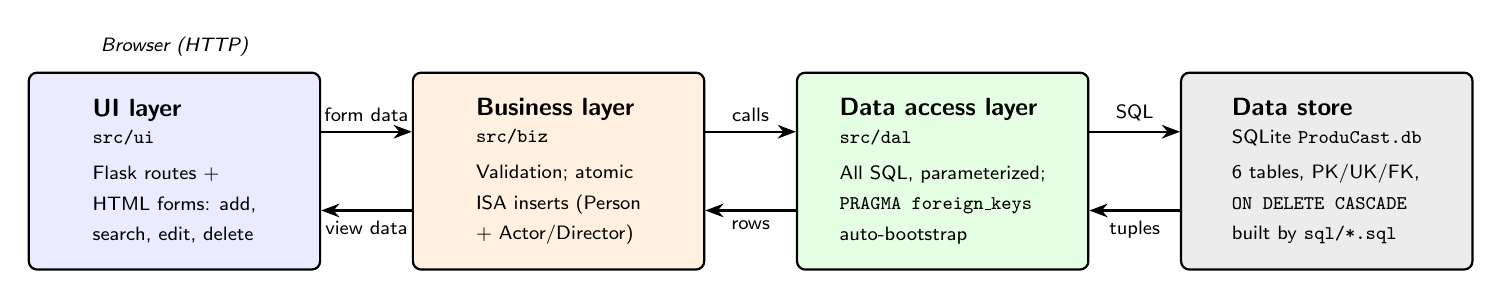
\begin{tikzpicture}[
  font=\sffamily\small, >=Stealth,
  layer/.style={draw, rounded corners=3pt, minimum width=3.7cm, minimum height=2.5cm, align=left, inner sep=4pt, thick},
  title/.style={font=\sffamily\small\bfseries, align=center},
  flow/.style={->, thick}]
 \node[layer, fill=blue!8]   (ui)  {\textbf{UI layer}\\[-1pt]\scriptsize\texttt{src/ui}\\[2pt]\scriptsize Flask routes +\\\scriptsize HTML forms: add,\\\scriptsize search, edit, delete};
 \node[layer, fill=orange!12, right=1.15cm of ui]  (biz) {\textbf{Business layer}\\[-1pt]\scriptsize\texttt{src/biz}\\[2pt]\scriptsize Validation; atomic\\\scriptsize ISA inserts (Person\\\scriptsize + Actor/Director)};
 \node[layer, fill=green!10, right=1.15cm of biz]  (dal) {\textbf{Data access layer}\\[-1pt]\scriptsize\texttt{src/dal}\\[2pt]\scriptsize All SQL, parameterized;\\\scriptsize \texttt{PRAGMA foreign\_keys}\\\scriptsize auto-bootstrap};
 \node[layer, fill=gray!15, right=1.15cm of dal]   (db) {\textbf{Data store}\\[-1pt]\scriptsize SQLite \texttt{ProduCast.db}\\[2pt]\scriptsize 6 tables, PK/UK/FK,\\\scriptsize \texttt{ON DELETE CASCADE}\\\scriptsize built by \texttt{sql/*.sql}};
 \draw[flow] ([yshift=.5cm]ui.east)  -- node[above,font=\sffamily\scriptsize]{form data} ([yshift=.5cm]biz.west);
 \draw[flow] ([yshift=-.5cm]biz.west)-- node[below,font=\sffamily\scriptsize]{view data} ([yshift=-.5cm]ui.east);
 \draw[flow] ([yshift=.5cm]biz.east) -- node[above,font=\sffamily\scriptsize]{calls} ([yshift=.5cm]dal.west);
 \draw[flow] ([yshift=-.5cm]dal.west)-- node[below,font=\sffamily\scriptsize]{rows} ([yshift=-.5cm]biz.east);
 \draw[flow] ([yshift=.5cm]dal.east) -- node[above,font=\sffamily\scriptsize]{SQL} ([yshift=.5cm]db.west);
 \draw[flow] ([yshift=-.5cm]db.west) -- node[below,font=\sffamily\scriptsize]{tuples} ([yshift=-.5cm]dal.east);
 \node[above=2pt of ui, font=\sffamily\scriptsize\itshape] {Browser (HTTP)};
\end{tikzpicture}}
\caption{System architecture. Requests flow left to right (UI $\rightarrow$ business $\rightarrow$ data access $\rightarrow$ SQLite) and results flow back; only the data layer contains SQL.}
\Description{Four boxes in a row labelled UI layer, business layer, data access layer and data store, with arrows in both directions between neighbours.}
\label{fig:arch}
\end{figure*}

\section{Populating and Querying the Database}
\textbf{Insertion.} \tn{02\_seed.sql} inserts people, subclasses and movies before their links, resolving names and titles instead of fixed IDs. The application also reuses existing people through parameterized lookup:
\begin{lstlisting}[language=SQLite]
SELECT Id FROM Person WHERE Name = ?;
INSERT INTO Person(Name) VALUES (?); -- if absent
\end{lstlisting}
\textbf{Retrieval.} Six queries in \tn{03\_queries.sql} are summarized in Table~\ref{tab:queries}. This query counts distinct directors per actor:
\begin{lstlisting}[language=SQLite]
SELECT P.Name, COUNT(DISTINCT MD.DirectorId) AS Directors
FROM Actor A JOIN Person P ON P.Id = A.PersonId
JOIN PerformanceRole R ON R.ActorId = A.Id
JOIN MovieDirector MD ON MD.MovieId = R.MovieId
GROUP BY A.Id, P.Name
HAVING COUNT(DISTINCT MD.DirectorId) > 1;
\end{lstlisting}
It returns DiCaprio (Nolan, Scorsese) and De Niro (Scorsese, Coppola); \tn{DISTINCT} prevents duplicate director counts.
\begin{table}[t]
\caption{Selected \tn{SELECT} queries and their results on the seeded database.}\label{tab:queries}
\footnotesize\setlength{\tabcolsep}{3pt}\begin{tabular}{@{}p{.9in}p{.8in}p{1.3in}@{}}\toprule
\textbf{Question} & \textbf{SQL features} & \textbf{Result}\\\midrule
Movies of one genre & \tn{WHERE}, \tn{LIKE} & Sci-Fi: \emph{Inception}, \emph{Star Wars}\\
Movies per director & \tn{JOIN}, \tn{GROUP BY} & Scorsese 2; five others 1\\
Cast size per movie & \tn{JOIN}, \tn{COUNT} & \emph{The Godfather} 2; others 1\\
Actors with several directors & \tn{HAVING}, \tn{DISTINCT} & DiCaprio 2, De Niro 2\\
Genres shared with Scorsese & subquery \tn{IN} & \emph{Raging Bull}, \emph{The Wolf of Wall Street}\\
Orphaned cast rows & \tn{LEFT JOIN}, \tn{IS NULL} & 0 rows (cascade check)\\\bottomrule
\end{tabular}
\end{table}
\textbf{Modification.} Updates and deletes use \tn{WHERE}; a representative test is:
\begin{lstlisting}[language=SQLite]
UPDATE Movie SET Genre = 'Science Fiction' WHERE Title = 'Star Wars';
DELETE FROM Movie WHERE Title = 'Star Wars';
\end{lstlisting}
Deleting \emph{Star Wars} changes Movie/MovieDirector/PerformanceRole counts from 7/7/8 to 6/6/7 without deleting people. Five tests reject a repeated person name, nonexistent director ID, invalid role type, repeated movie--actor pair and null title.


\begin{figure*}[t]
\centering
\uishot{ui_entry.png}{Insertion: Network Data Entry forms (one per multi-table insert).}\hfill
\uishot{ui_portfolio.png}{Retrieval: Project Portfolio with its movies and directors.}\\[3pt]
\uishot{ui_roster.png}{Management: Talent Rosters for the \tn{Person} IS-A hierarchy (rename, delete).}\hfill
\uishot{ui_ledger.png}{Result: Casting Ledger showing the \tn{PerformanceRole} bridge.}
\caption{The web application in use: insertion (a), portfolio retrieval (b), roster management (c) and ledger results (d).}
\Description{Four screenshots of the web application: data entry forms, a movie list, director and actor rosters, and the casting ledger.}
\label{fig:ui}
\end{figure*}

\section{User Interface}
Figure~\ref{fig:ui} shows four workflows. The Network Data Entry page (a) creates records through forms rather than requiring users to enter IDs. The Project Portfolio (b) lists movies and associated directors; Talent Rosters (c) expose actor and director records for editing or deletion. The Casting Ledger (d) displays movie--actor assignments with their character and role types. Input passes through the business layer, where services resolve entered names and titles to stored identifiers. Thus, the interface exposes the relationships in the ER model without presenting raw SQL to the user.

\section{Design Decisions}
Surrogate \tn{Id} keys simplify joins while unique names/titles prevent duplicates. Cascading deletes avoid manually removing orphaned links. \tn{CHECK} restricts \tn{RoleType}; service validation rejects empty strings that \tn{NOT NULL} permits. Forms accept names and titles, which services resolve to IDs. This keeps displayed values readable while foreign keys retain stable links. The separation of routes, services and SQL also localizes data-integrity checks: a failed validation is reported before an invalid multi-table change is committed.

\section{Validation of the Mapping}
The sample uses six relations with 12 people, seven movies and eight cast links (Table~\ref{tab:rows}). The director-count query traverses the performance and directing bridges; \tn{DISTINCT} prevents duplicate counting and identifies DiCaprio and De Niro with two directors each. The orphan query returns no rows. Updating a movie's genre preserves its links, while deleting \emph{Star Wars} removes its two dependent links but leaves people intact. Five rejection cases test duplicate names, missing directors, invalid roles, duplicate assignments and null titles. These checks demonstrate the principal constraints for the seeded instance, not exhaustive coverage.

\section{Reproducibility and Discussion}
The repository provides scripts, source, diagrams, screenshots and setup instructions, following FAIR~\cite{fair}. Install with \tn{pip install -r requirements.txt}; \tn{python main.py} initializes and seeds the database, \tn{--reset} rebuilds it and \tn{--queries} runs examples. An earlier submission failed because a working-directory-dependent path created an empty SQLite database; corrected paths now pass tests from four directories.
\textbf{Mapping limits.} Keys and participation constraints carry over, but relationship labels and overlapping IS-A meaning are not explicit in SQL. Unique names and one role per movie are assumptions; RDF/OWL in Part~II will describe the semantics.
\textbf{Contributions and AI.} K.B. developed the conceptual model/IS-A mapping; M.P. built the relational implementation. Gemini~\cite{gemini} generated an initial implementation that failed demonstration; Claude~\cite{claude} refactored the layers and drafted scripts and report. We validated its output with tests because it could not access the repository.



\begin{thebibliography}{9}
\bibitem{iso} ISO/IEC. 2023. ISO/IEC 9075:2023 Information technology -- Database languages SQL.
\bibitem{sqlite} SQLite Consortium. 2026. SQLite. https://www.sqlite.org.
\bibitem{fair} Mark D. Wilkinson et al. 2016. The FAIR Guiding Principles for scientific data management and stewardship. \emph{Scientific Data} 3 (2016), 160018.
\bibitem{claude} Anthropic. 2026. Claude. AI help with refactoring, SQL scripts and report drafting.
\bibitem{gemini} Google. 2026. Gemini. AI help with the first implementation.
\end{thebibliography}

\clearpage
\begin{table*}[p]
\caption{All relations, attributes and constraints (DDL in \tn{src/dal/models/relational/sql/01\_schema.sql}). PK = primary key
(\tn{INTEGER PRIMARY KEY AUTOINCREMENT}), UK = candidate key, FK = foreign key, CK = \tn{CHECK}. ER origin gives the ERD construct each relation implements.}
\label{tab:schema}
\small\renewcommand{\arraystretch}{1.45}\setlength{\tabcolsep}{3pt}
\begin{tabular}{@{}p{1.0in}p{.8in}p{.9in}p{.35in}p{.45in}>{\raggedright\arraybackslash}p{3.0in}@{}}\toprule
\textbf{Relation (ER origin)} & \textbf{Attribute} & \textbf{Type} & \textbf{Null} & \textbf{Key} & \textbf{Constraint / meaning}\\\midrule
\tn{Person} (entity set; IS-A superclass) & \tn{Id} & INTEGER & no & PK & surrogate key\\
 & \tn{Name} & VARCHAR(255) & no & UK & \tn{UK\_\allowbreak Person\_\allowbreak Name UNIQUE (Name)}: natural key\\\midrule
\tn{Actor} (subclass IS-A) & \tn{Id} & INTEGER & no & PK & surrogate key\\
 & \tn{PersonId} & INTEGER & no & FK, UK & \tn{FK\_\allowbreak Actor\_\allowbreak PersonId\_\allowbreak 2\_\allowbreak Person\_\allowbreak Id} (CASCADE); \tn{UK\_\allowbreak Actor\_\allowbreak PersonId} (1:1 mapping)\\\midrule
\tn{Director} (subclass IS-A) & \tn{Id} & INTEGER & no & PK & surrogate key\\
 & \tn{PersonId} & INTEGER & no & FK, UK & \tn{FK\_\allowbreak Director\_\allowbreak PersonId\_\allowbreak 2\_\allowbreak Person\_\allowbreak Id} (CASCADE); \tn{UK\_\allowbreak Director\_\allowbreak PersonId} (1:1 mapping)\\\midrule
\tn{Movie} (entity set) & \tn{Id} & INTEGER & no & PK & surrogate key\\
 & \tn{Title} & VARCHAR(255) & no & UK & \tn{UK\_\allowbreak Movie\_\allowbreak Title UNIQUE (Title)}: natural key\\
 & \tn{Genre} & VARCHAR(255) & no & & mandatory text\\
 & \tn{StudioName} & VARCHAR(255) & yes & & optional\\\midrule
\tn{MovieDirector} (M:N bridge, Movie--Director) & \tn{Id} & INTEGER & no & PK & surrogate key\\
 & \tn{MovieId} & INTEGER & no & FK & \tn{FK\_\allowbreak MovieDirector\_\allowbreak MovieId\_\allowbreak 2\_\allowbreak Movie\_\allowbreak Id} (CASCADE)\\
 & \tn{DirectorId} & INTEGER & no & FK & \tn{FK\_\allowbreak MovieDirector\_\allowbreak DirectorId\_\allowbreak 2\_\allowbreak Director\_\allowbreak Id} (CASCADE)\\
 & & & & UK & \tn{UK\_\allowbreak MovieDirector\_\allowbreak MovieId\_\allowbreak DirectorId UNIQUE (MovieId, DirectorId)}\\\midrule
\tn{PerformanceRole} (M:N bridge, ERD \tn{Performance\_\allowbreak Role}) & \tn{Id} & INTEGER & no & PK & surrogate key\\
 & \tn{MovieId} & INTEGER & no & FK & \tn{FK\_\allowbreak PerformanceRole\_\allowbreak MovieId\_\allowbreak 2\_\allowbreak Movie\_\allowbreak Id} (CASCADE)\\
 & \tn{ActorId} & INTEGER & no & FK & \tn{FK\_\allowbreak PerformanceRole\_\allowbreak ActorId\_\allowbreak 2\_\allowbreak Actor\_\allowbreak Id} (CASCADE)\\
 & \tn{RoleName} & VARCHAR(255) & no & & the character played\\
 & \tn{RoleType} & VARCHAR(20) & no & CK & \tn{DEFAULT 'Supporting'}; \tn{CK\_\allowbreak PerformanceRole\_\allowbreak RoleType CHECK (RoleType IN ('Lead','Supporting','Cameo'))}\\
 & & & & UK & \tn{UK\_\allowbreak PerformanceRole\_\allowbreak MovieId\_\allowbreak ActorId UNIQUE (MovieId, ActorId)} (one role per actor and movie)\\\bottomrule
\end{tabular}

\medskip\raggedright
\textbf{Referential integrity.} Foreign-key enforcement is enabled on every connection (\tn{PRAGMA foreign\_keys = ON}) by \tn{database.get\_connection}.
All foreign keys use \tn{ON DELETE CASCADE}: deleting a \tn{Person} removes its \tn{Actor}/\tn{Director} rows and their links; deleting a
\tn{Movie} removes only its \tn{MovieDirector} and \tn{PerformanceRole} rows. Movies and people are never deleted by cascade from a link.\\
\textbf{Mapping assumptions.} The specialization is overlapping (a person may have both an \tn{Actor} and a \tn{Director} row) and the
application always creates the subclass row together with its \tn{Person} row. Movies, actors and directors may exist before their
links, but every link row must reference existing parents. A movie may have several directors or none; an actor has at most one role per movie.\\
\textbf{Implementation checks.} Each \tn{Id} is \tn{INTEGER PRIMARY KEY AUTOINCREMENT} and each foreign key is \tn{INTEGER}. \tn{NOT NULL} does not reject
empty strings, so the business layer rejects blank values before they reach the database. The DDL and this report agree on keys, \tn{NULL} values and cascading deletion.\\
\textbf{Loaded instance.} Person 12 $\cdot$ Actor 6 $\cdot$ Director 6 $\cdot$ Movie 7 $\cdot$ MovieDirector 7 $\cdot$ PerformanceRole 8.
\end{table*}
\end{document}